% Chapter 5: RL in Games

With multiple agents adapting simultaneously, each agent's environment includes the others' changing policies, so the stationary-transition assumption behind single-agent convergence results fails. \citet{shoham2007multiagent} enumerate five desiderata for multi-agent learning: (1) convergence to a stationary strategy in self-play; (2) rationality (best-responding against stationary opponents); (3) equilibrium attainment; (4) safety (guaranteeing at least the Nash-value payoff); (5) social welfare. No existing algorithm satisfies all five in general games.

Two paradigms emerged. Value-based methods generalize the Bellman operator to games, replacing the $\max$ with game-theoretic solution concepts (minimax, Nash), targeting stochastic games with simultaneous moves and observable payoffs. Regret-based methods (CFR) accumulate counterfactual regrets and let the time-averaged strategy converge, targeting extensive-form games with sequential moves and private information. Computing Nash equilibria is PPAD-complete \citep{Daskalakis2009}, so neither approach escapes the fundamental hardness, but both achieve convergence in the game classes they target.

\subsection{Stochastic Games and Equilibrium Learning}

\subsubsection{The Stochastic Game Framework}

An $n$-player stochastic game $\Gamma = (n, \mathcal{S}, \mathcal{A}_1, \ldots, \mathcal{A}_n, P, r_1, \ldots, r_n, \gamma)$ consists of a finite state space $\mathcal{S}$; finite action sets $\mathcal{A}_i$ for each player $i$; a transition function $P: \mathcal{S} \times \mathcal{A}_1 \times \cdots \times \mathcal{A}_n \to \Delta(\mathcal{S})$; reward functions $r_i: \mathcal{S} \times \mathcal{A}_1 \times \cdots \times \mathcal{A}_n \to \mathbb{R}$; and a common discount factor $\gamma \in [0,1)$. At each stage, all players simultaneously choose actions, receive individual rewards, and the game transitions to a new state.\footnote{\citet{shapley1953stochastic} introduced stochastic games in 1953 for the two-player zero-sum case, proving existence of the value via a contraction argument on the Bellman operator. The general-sum extension to $n$ players is due to Fink (1964) and Takahashi (1964).}

A Markov decision process is a stochastic game with $n = 1$; a matrix game is a stochastic game with $|\mathcal{S}| = 1$. Each player $i$ seeks a policy $\pi_i: \mathcal{S} \to \Delta(\mathcal{A}_i)$ maximizing discounted return $\mathbb{E}[\sum_{t=0}^\infty \gamma^t r_i(s_t, a_{1,t}, \ldots, a_{n,t})]$.

Standard Q-learning convergence \citep{WatkinsDayan1992} requires stationary transition and reward dynamics; with multiple learners, this assumption fails. \citet{BowlingVeloso2002} formalized two properties a learning algorithm should satisfy. It is \emph{rational} if, when all other players converge to stationary policies, it converges to a best response; it is \emph{convergent} if, in self-play, it converges to a stationary policy.

If all players use rational, convergent algorithms, the resulting profile is a Nash equilibrium by construction. The challenge is achieving both properties simultaneously.

\subsubsection{Minimax-Q Learning}

\citet{littman1994markov} proposed the first Q-learning algorithm for stochastic games, targeting two-player zero-sum games. The key modification replaces the $\max$ operator in the standard Q-learning backup with a minimax operator. Each agent maintains $Q_i(s, a_i, a_{-i})$ over the joint action space. The update rule is
\begin{equation}
Q_i(s, a_i, a_{-i}) \leftarrow (1-\alpha)\, Q_i(s, a_i, a_{-i}) + \alpha\left[r_i + \gamma\, V_i(s')\right],
\end{equation}
where the value backup solves a linear program:
\begin{equation}
V_i(s) = \max_{\pi_i \in \Delta(\mathcal{A}_i)} \min_{a_{-i} \in \mathcal{A}_{-i}} \sum_{a_i \in \mathcal{A}_i} \pi_i(a_i)\, Q_i(s, a_i, a_{-i}).
\label{eq:minimaxv}
\end{equation}
This is the RL analogue of Shapley's value iteration for zero-sum stochastic games \citep{Shapley1964}. The resulting policy $\pi_i(s)$ is generally a mixed strategy, since deterministic policies are exploitable in adversarial settings.

Minimax-Q converges to the minimax Q-values under Robbins-Monro learning rates ($\sum_t \alpha_t = \infty$, $\sum_t \alpha_t^2 < \infty$) and infinite exploration of all state-action tuples.\footnote{The convergence proof extends the contraction argument for standard Q-learning. Because the zero-sum minimax operator is a contraction with modulus $\gamma$ under the $\ell^\infty$ norm, the stochastic approximation converges to the fixed point. See \citet{littman1994markov} and the general treatment in Szepesvári and Littman (1999).} However, the algorithm sacrifices rationality: it plays the equilibrium strategy even against exploitable opponents.\footnote{In the soccer game of \citet{littman1994markov}, minimax-Q won 53.7\% against a hand-built opponent versus 26.1\% for Q-learning. Against an adversarial challenger, Q-learning won 0\% (its deterministic policy was fully predictable); minimax-Q won 37.5\% through mixed strategies.}

\subsubsection{Nash-Q Learning}

\citet{hu2003nash} extended the framework to general-sum stochastic games, where players may have aligned, opposed, or mixed incentives. Each agent $i$ maintains a Q-function over the joint action space $Q_i(s, a_1, \ldots, a_n)$ and updates via
\begin{equation}
Q_i(s, \mathbf{a}) \leftarrow (1-\alpha)\, Q_i(s, \mathbf{a}) + \alpha\left[r_i + \gamma\, \text{Nash}_i\bigl(Q_1(s'), \ldots, Q_n(s')\bigr)\right],
\end{equation}
where $\text{Nash}_i(\cdot)$ denotes player $i$'s payoff under a Nash equilibrium of the stage game defined by the current Q-values $(Q_1(s'), \ldots, Q_n(s'))$. At each backup, the algorithm treats the Q-values as payoff matrices, computes a Nash equilibrium of this matrix game, and uses the equilibrium payoffs for the value estimate.

\begin{theorem}[\citet{hu2003nash}]
Nash-Q converges to Nash Q-values under Robbins-Monro learning rates and infinite exploration, provided every stage game encountered during learning has either (a) a global optimal point (all agents receive their highest payoff at the same joint action) or (b) a unique saddle-point Nash equilibrium.
\end{theorem}

These conditions are restrictive. When stage games have multiple Nash equilibria, agents may select different equilibria for their backups, causing divergence.\footnote{In the experiments of \citet{hu2003nash}, a grid game with a unique equilibrium Q-function converged in 100\% of trials under Nash-Q versus 20\% under independent Q-learning; a game with three equilibrium Q-functions converged in only 68--90\% of trials. Nash-Q requires each agent to observe all other agents' rewards and to maintain Q-values over the joint action space $\mathcal{A}_1 \times \cdots \times \mathcal{A}_n$, with storage $O(n |\mathcal{S}| \prod_i |\mathcal{A}_i|)$, exponential in the number of players.} Nash-Q reduces to standard Q-learning in the single-agent case.

\subsubsection{The Convergence Problem}

Table~\ref{tab:marl_comparison} summarizes the trade-offs. No single algorithm achieves both rationality and convergence in general games.

\begin{table}[htbp]
\centering
\caption{Multi-agent Q-learning algorithms: convergence and information requirements}
\label{tab:marl_comparison}
\begin{tabular}{l cc ll}
\hline
Algorithm & Rational & Convergent & Game class & Information \\
\hline
Indep.\ Q-learning & Yes & No & Any & Own reward \\
Minimax-Q & No & Yes & Zero-sum & Joint actions \\
Nash-Q & Cond. & Cond. & General-sum & All rewards \\
WoLF-PHC & Yes & Yes ($2{\times}2$) & General-sum & Own reward \\
\hline
\end{tabular}
\end{table}

WoLF-PHC (Win or Learn Fast, Policy Hill-Climbing) of \citet{BowlingVeloso2002} maintains a policy $\pi_i(a|s)$ and a running average policy $\bar{\pi}_i(a|s)$, updating Q-values as in standard Q-learning. The policy moves toward the greedy action at a variable rate:
\begin{equation}
\delta = \begin{cases}
\delta_l & \text{if } \sum_a \pi_i(a|s)\, Q_i(s,a) < \sum_a \bar{\pi}_i(a|s)\, Q_i(s,a) \quad \text{(losing)} \\
\delta_w & \text{otherwise} \quad \text{(winning)}
\end{cases}
\end{equation}
with $\delta_l > \delta_w$. When the current policy underperforms the historical average (losing), the agent adapts quickly; when outperforming (winning), it adapts slowly to avoid destabilizing the opponent. \citet{BowlingVeloso2002} proved that WoLF-IGA (the infinitesimal gradient ascent variant) converges to Nash equilibrium in all two-player, two-action games. The trajectory traces piecewise ellipses around the equilibrium, shrinking by a factor of $\ell^4 < 1$ per orbit, where $\ell = \sqrt{\delta_w / \delta_l}$. WoLF-PHC requires only own-reward observations, the same information as independent Q-learning.

Two further algorithms deserve mention. Friend-or-Foe Q-learning \citep{littman2001friend} decomposes agents as cooperative (friend) or adversarial (foe), using $\max$ for friends and minimax for foes; it always converges but requires knowing the relationship type a priori.\footnote{Correlated-Q learning \citep{greenwald2003correlated} generalizes both Nash-Q and Minimax-Q by using correlated equilibrium, a probability distribution over joint actions enforced by a correlating device. The set of correlated equilibria contains all Nash equilibria. Correlated-Q converges under conditions analogous to Nash-Q.} The evolutionary perspective of \citet{borgers1997learning} provides a deeper lens: reinforcement learning dynamics in matrix games converge to the replicator equation from evolutionary game theory. The cycling of Q-learning in games such as matching pennies is structurally identical to the cycling of replicator dynamics in Rock-Paper-Scissors games.

\subsubsection{Simulation Study: Cournot and Bertrand Duopoly}
\label{sec:cournot_bertrand}

Two canonical games from industrial organization serve as benchmarks. In Cournot duopoly, two firms choose quantities $q_i \in \{0, 1, \ldots, 9\}$ with inverse demand $P(Q) = 10 - Q$ and marginal cost $c = 1$; the continuous Nash equilibrium is $q^* = 3$ with profit $\pi^* = 9$. In Bertrand duopoly with differentiated products, two firms choose prices $p_i \in \{0, 1, \ldots, 9\}$ with demand $d_i = 10 - 2 p_i + p_j$ and marginal cost $c = 1$; the symmetric first-order condition gives $p^* = (a + b c)/(2 b - e) = 4$ with profit $\pi^* = 18$. Bertrand admits a single pure-strategy Nash on the integer grid at $(p_0, p_1) = (4, 4)$, while Cournot admits three pure-strategy Nash equilibria on the integer grid, $(2, 4)$, $(3, 3)$, and $(4, 2)$, only the symmetric of which coincides with the continuous solution.\footnote{Each configuration runs for 50,000 iterations across 20 seeds. The Nash-Q implementation here selects the joint-payoff-maximizing equilibrium when multiple pure Nash exist, a deviation from the canonical Hu-Wellman 2003 backup that pins down a single value function; in this game it picks $(3, 3)$ for Cournot.} Three algorithms compete: independent Q-learning (IQL), Nash-Q, and WoLF-PHC. The framing connects to the recent literature on Q-learning collusion in IO duopoly \citep{Calvano2020}; the stateless design used here has no memory of past actions, so collusive trigger strategies are not available and the equilibria reached are one-shot Nash.

\begin{table}[htbp]
\centering
\caption{Convergence to Nash equilibrium in Cournot and Bertrand duopoly}
\label{tab:cournot_bertrand}
\begin{tabular}{ll rr r}
\hline
Game & Algorithm & Action & Profit & $|a - a^*|$ \\
\hline
Cournot & IQL & $2.95 \pm 0.05$ & $9.1 \pm 0.0$ & $0.05$ \\
 & Nash-Q & $2.89 \pm 0.33$ & $8.8 \pm 1.3$ & $0.17$ \\
 & WoLF-PHC & $3.00 \pm 0.00$ & $9.0 \pm 0.0$ & $0.00$ \\
\hline
Bertrand & IQL & $4.00 \pm 0.00$ & $18.0 \pm 0.0$ & $0.00$ \\
 & Nash-Q & $4.00 \pm 0.00$ & $18.0 \pm 0.0$ & $0.00$ \\
 & WoLF-PHC & $3.95 \pm 0.05$ & $17.8 \pm 0.2$ & $0.05$ \\
\hline
\end{tabular}
\begin{minipage}{0.9\textwidth}
\footnotesize
Notes: Action and Profit report mean $\pm$ standard error across 20 seeds over the final 5,000 iterations. $|a - a^*|$ is the mean distance from the symmetric continuous Nash action ($q^* = 3$ for Cournot, $p^* = 4$ for Bertrand).
\end{minipage}
\end{table}

Table~\ref{tab:cournot_bertrand} and Figure~\ref{fig:cournot_bertrand} report the results. All three algorithms settle near the symmetric Nash in both games. IQL, which lacks any game-theoretic computation, matches the game-aware methods in these well-structured games. The advantage of Nash-Q and WoLF-PHC emerges in games requiring mixed strategies, where IQL's deterministic policy limit prevents convergence.

\begin{figure}[htbp]
\centering
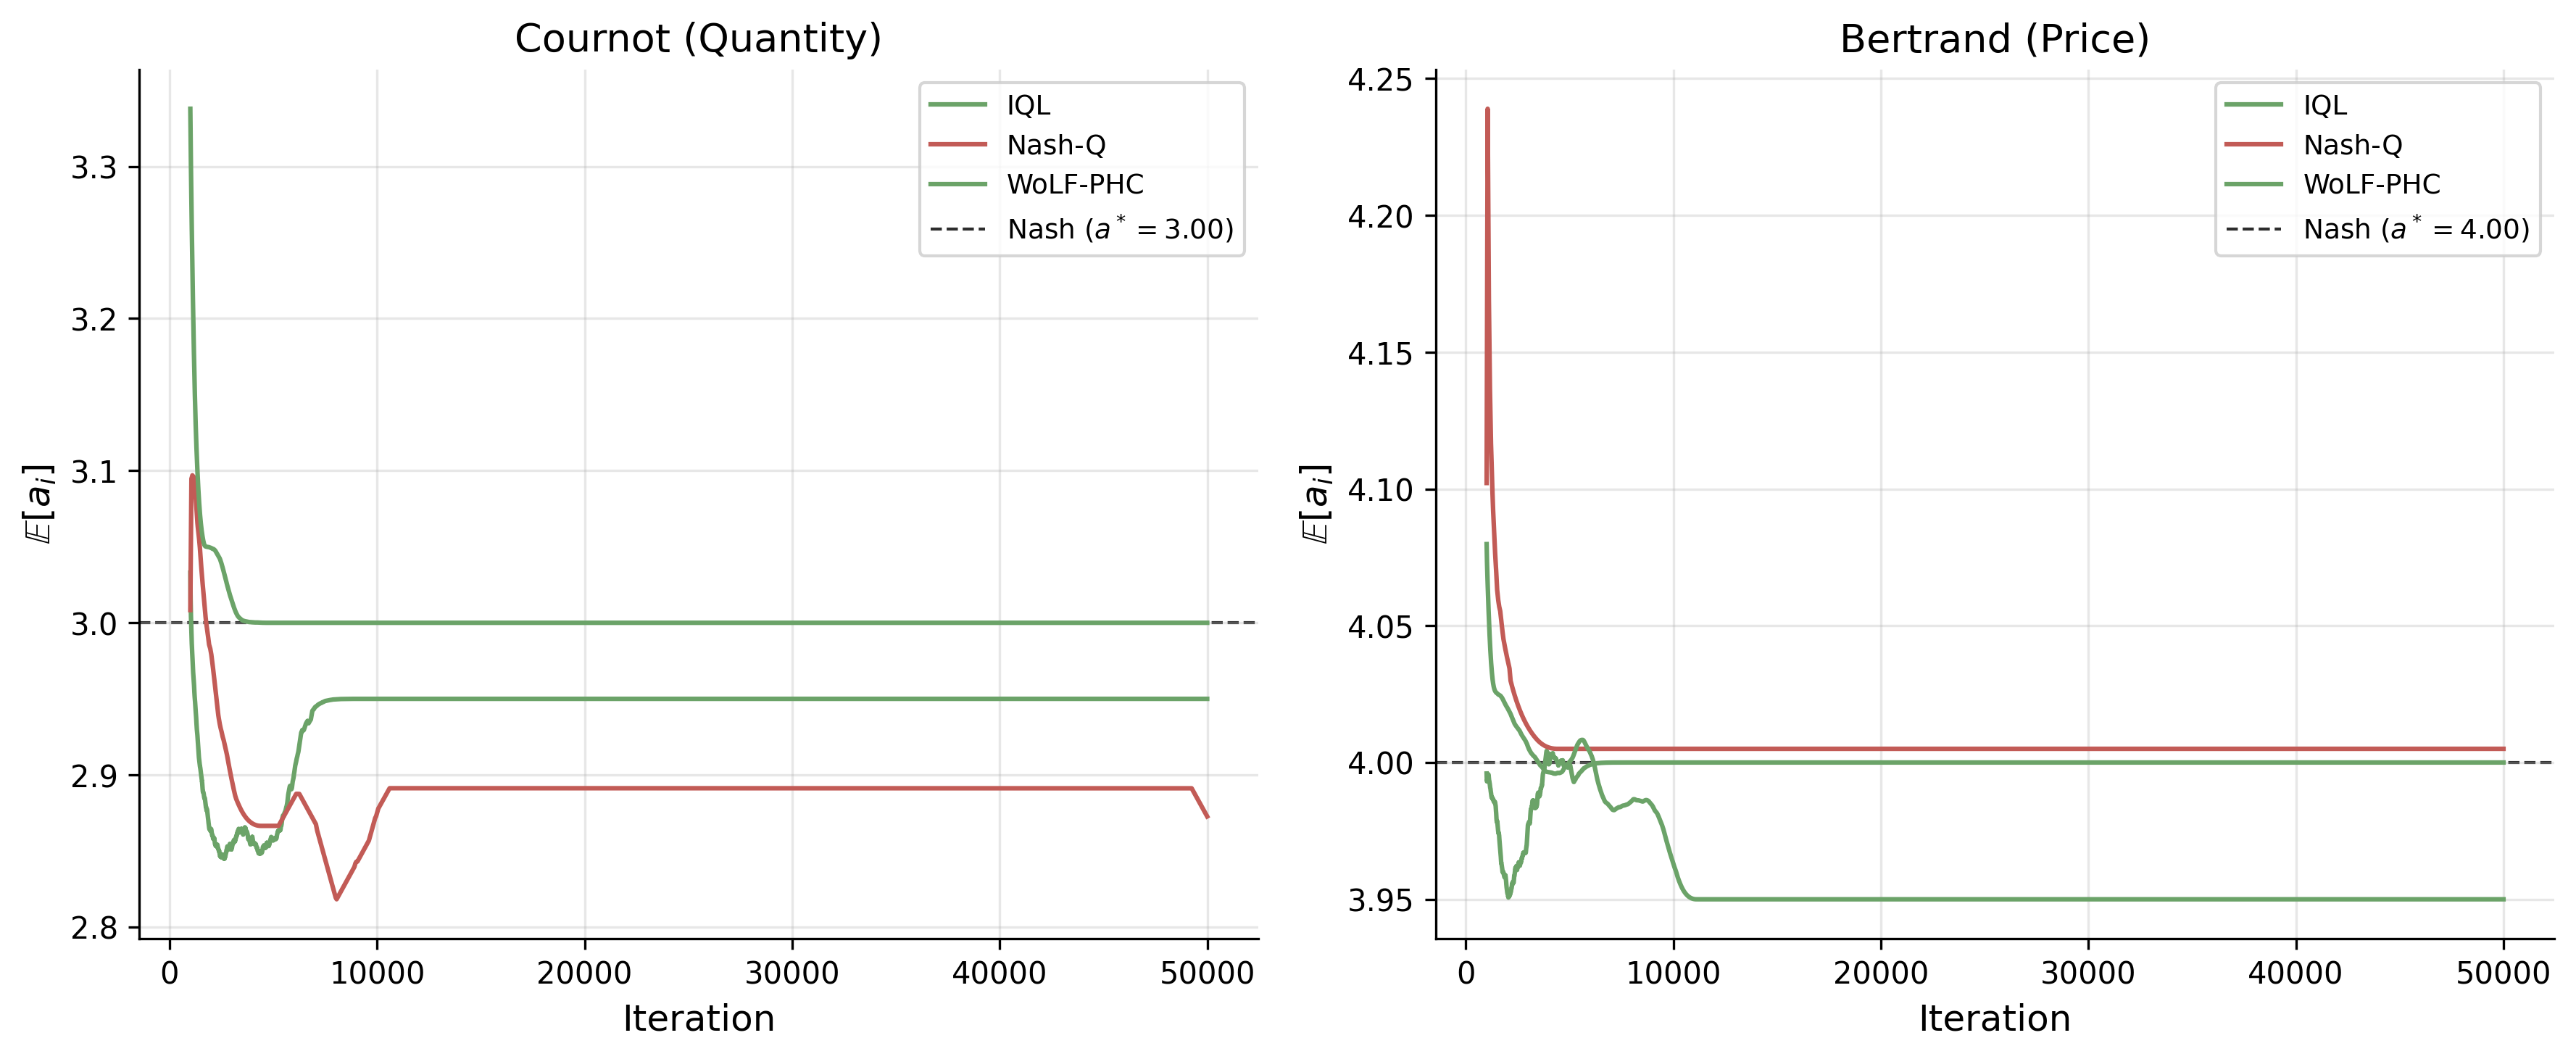
\includegraphics[width=\textwidth]{../ch06_games/sims/cournot_bertrand_marl.png}
\caption{Convergence of expected actions to Nash equilibrium. Left: Cournot duopoly. Right: Bertrand duopoly. Smoothed over 1,000-iteration windows, averaged across 20 seeds.}
\label{fig:cournot_bertrand}
\end{figure}

\subsection{Counterfactual Regret Minimization}

Extensive-form games require a different approach. CFR bypasses equilibrium selection: instead of computing Nash equilibria at each step, it minimizes cumulative regret and lets the time-averaged strategy converge to equilibrium.

An extensive-form game consists of a game tree with information sets $\mathcal{I}_i$ partitioning player $i$'s decision nodes. An information set groups nodes where the player cannot distinguish between them due to hidden opponent actions or private information. A behavioral strategy $\sigma_i: \mathcal{I}_i \to \Delta(\mathcal{A})$ assigns action probabilities at each information set.

The \emph{counterfactual value} of action $a$ at information set $I$ is
\begin{equation}
v^\sigma_i(I, a) = \sum_{h \in I} \pi^\sigma_{-i}(h) \sum_{z \sqsupseteq ha} \pi^\sigma(ha, z) u_i(z)
\end{equation}
where $\pi^\sigma_{-i}(h)$ is the probability opponents reach $h$, and $\pi^\sigma(ha, z)$ is the probability of reaching terminal $z$ from $ha$. The counterfactual formulation weights by opponent reach $\pi^\sigma_{-i}(h)$ rather than joint reach $\pi^\sigma(h)$, ensuring non-zero updates even at rarely-visited information sets. Cumulative regret for action $a$ is $R^T(I,a) = \sum_{t=1}^T [v^{\sigma^t}(I,a) - v^{\sigma^t}(I)]$. CFR updates via \emph{regret matching}:\footnote{Regret matching is an action selection rule where the probability of choosing action $a$ is proportional to the cumulative regret for not having chosen $a$ in the past (truncated at zero). Actions with high regret receive higher probability; actions with negative regret (having performed worse than average) receive zero probability.}
\begin{equation}
\sigma^{T+1}(I, a) = \frac{[R^T(I, a)]^+}{\sum_{a'} [R^T(I, a')]^+}, \quad [x]^+ = \max(x,0).
\end{equation}
The average strategy $\bar{\sigma}^T$ converges to $\varepsilon$-Nash with $\varepsilon = O(|\mathcal{I}|\sqrt{|\mathcal{A}|}\Delta / \sqrt{T})$, where $\Delta$ is the range of payoffs \citep{zinkevich2008}.\footnote{An $\varepsilon$-Nash equilibrium is a strategy profile where no player can improve her expected payoff by more than $\varepsilon$ through unilateral deviation. As $\varepsilon \to 0$, this converges to an exact Nash equilibrium.}

CFR+ \citep{tammelin2014solving} replaces standard regret matching with Regret Matching+, which truncates cumulative regrets to zero after each update rather than only at action selection. The update becomes $R^{T+1}(I, a) = \max(R^T(I, a) + r^{T+1}(I, a),\, 0)$, where $r^{T+1}(I,a) = v^{\sigma^{T+1}}(I,a) - v^{\sigma^{T+1}}(I)$ is the instantaneous counterfactual regret. CFR+ also weights iteration $t$ by $t$ when computing the average strategy. While vanilla CFR converges at $O(1/\sqrt{T})$, CFR+ empirically converges at $O(1/T)$.\footnote{The $O(1/T)$ rate for CFR+ is empirically observed but not yet proven in full generality. \citet{tammelin2014solving} conjectured this rate based on extensive experiments across poker variants.} CFR+ enabled \citet{bowling2015heads} to essentially solve heads-up limit Texas hold'em, a game with $3.16 \times 10^{17}$ states, the first non-trivial imperfect-information game played competitively by humans to be essentially solved. Their program Cepheus achieved exploitability below 1 mbb/g (milli-big-blind per game).

\subsection{Neural Extensions}

Tabular CFR stores regrets at every information set, infeasible when $|\mathcal{I}| > 10^{14}$. Two neural approaches scale to large games.

\subsubsection{Deep CFR}

\citet{Brown2019} approximate cumulative regrets with a neural network $V_\theta: \mathcal{I} \times \mathcal{A} \to \mathbb{R}$ trained on sampled (information set, iteration, regret) tuples:
\begin{equation}
L_V(\theta) = \mathbb{E}_{(I, t', r) \sim \mathcal{M}} \left[ t' \cdot (V_\theta(I, a) - r)^2 \right].
\end{equation}
Weighting by iteration index $t'$ gives more recent regret estimates higher importance.
A separate network $\Pi_\phi$ approximates the average strategy, trained via weighted MSE on strategy samples with the same iteration weighting. The current strategy derives from regret matching, with $\sigma(I, a) \propto [V_\theta(I, a)]^+$.

\subsubsection{Neural Fictitious Self-Play}

NFSP \citep{heinrich2016deep} combines \emph{fictitious play}\footnote{Fictitious play \citep{Brown1951} is a classical learning rule where each player best-responds to the empirical distribution of opponents' past actions. Under certain conditions (e.g., two-player zero-sum games), the time-average strategies converge to Nash equilibrium.} \citep{Brown1951} with deep Q-learning.\footnote{Deep Q-Network (DQN) \citep{mnih2015} approximates the Q-function with a neural network, using experience replay and a target network to stabilize training. The target network $\theta^-$ in the loss function is a delayed copy of the main network, updated periodically.} Each player maintains two networks: a best-response network $Q_\theta$ trained via DQN, and an average strategy network $\bar{\pi}_\phi$ trained via supervised learning on the best-response actions:
\begin{equation}
L_{\text{RL}}(\theta) = \mathbb{E}\left[ \left( r + \gamma \max_{a'} Q_{\theta^-}(I', a') - Q_\theta(I, a) \right)^2 \right], \quad
L_{\text{SL}}(\phi) = \mathbb{E}\left[ -\log \bar{\pi}_\phi(a | I) \right].
\end{equation}
During play, agents follow $\bar{\pi}_\phi$ with probability $1-\eta$ and $Q_\theta$ with probability $\eta$.

\subsubsection{Poker Results}

These methods achieved superhuman performance in poker. Deep CFR attained \emph{exploitability} of 37 mbb/g\footnote{Exploitability measures how far a strategy is from Nash equilibrium, defined as the maximum expected gain an adversary could achieve by best-responding. Zero exploitability means the strategy is unexploitable (Nash). In poker, exploitability is measured in milli-big-blinds per game (mbb/g).} in heads-up flop hold'em \citep{Brown2019}. Libratus defeated top human professionals in heads-up no-limit hold'em using nested subgame solving with CFR \citep{brown2017superhuman}. Pluribus extended to six-player no-limit hold'em \citep{brown2019superhuman}. The game tree of heads-up no-limit hold'em contains $\sim 10^{161}$ states; these results demonstrate that CFR-based methods scale to practically relevant game sizes.

\subsection{The Coase Conjecture in a Durable Goods Monopoly}
\label{subsec:coase}

The durable goods monopoly is a canonical extensive-form bargaining problem with private information: the seller does not know the buyer's valuation.

\citet{coase1972durability} conjectured that a durable goods monopolist\footnote{A durable good provides utility over multiple periods (e.g., a car, appliance, or software license) rather than being consumed immediately. Unlike non-durable goods, durable goods create intertemporal competition, as the seller at time $t$ competes with her own future self at $t+1$.} loses market power when buyers are patient. Unable to commit to future prices, the seller competes with her future self, eroding rents. As the inter-offer interval shrinks ($\delta \to 1$), price collapses to marginal cost and all surplus is extracted by buyers. \citet{stokey1981rational} showed that a monopolist facing rational consumers cannot price discriminate intertemporally; \citet{bulow1982durable} proved that in the no-gap case the monopolist prefers renting to selling. \citet{gul1986foundations} formalized the Coase conjecture for the gap case, where the seller's cost is strictly below all buyer valuations, establishing that the unique stationary Markov-perfect equilibrium price collapses to marginal cost as the period length shrinks. \citet{ausubel1989reputation} and the survey of \citet{ausubel2002bargaining} extend the analysis to the no-gap case and to bargaining with two-sided incomplete information.

The Coase conjecture is asymptotic in $T$ and $\delta$. A two-period game cannot exhibit it; the surplus erosion only operates when the seller can re-optimize many times and buyers can credibly wait. The simulation below uses backward induction on the seller's recursive problem with a continuum of buyers, varying $T$ and $\delta$ on a grid, and compares the Markov-perfect no-commitment value against the commitment benchmark. A separate two-period simulation in Section~\ref{subsec:durable_goods_screening} illustrates the screening-versus-pooling equilibrium structure that underlies the durable-goods game; the Coase conjecture proper is delivered by the asymptotic sweep here.

\subsubsection{Model and Dynamic Programming}

A monopolist with marginal cost $c = 0$ faces a continuum of buyers with valuations $v$ drawn from the uniform distribution on $[0, 1]$. The mass of buyers is normalized to one. In each period $t = 1, \ldots, T$, the seller posts a price $p_t$; each remaining buyer of type $v$ accepts iff $v - p_t \ge \delta \, \mathbb{E}_t[v - p_{t+1}^*]$, where $p_{t+1}^*$ is the equilibrium price the seller will post at $t+1$. The seller's per-period revenue is $p_t$ times the mass of buyers who accept.

Define the state at the start of period $t$ as the cutoff $v_t \in [0, 1]$: remaining buyers have valuations uniformly distributed on $[0, v_t]$, with mass $v_t$. The seller's action is the next-period cutoff $w \in [0, v_t]$; buyers with type in $[w, v_t]$ accept at price $p_t$ and exit, while those in $[0, w]$ remain. Marginal-buyer indifference at $w$ pins down the posted price,
\begin{equation}
p_t(w) = (1 - \delta) w + \delta \, p_{t+1}^*(w),
\label{eq:coase_marginal_price}
\end{equation}
where $p_{t+1}^*(w)$ is the seller's equilibrium price at state $w$ in period $t+1$. The seller's Bellman equation is
\begin{equation}
V_t(v) = \max_{w \in [0, v]} \left\{ p_t(w) \, (v - w) + \delta \, V_{t+1}(w) \right\},
\label{eq:coase_bellman}
\end{equation}
with terminal condition $V_T(v) = \max_{w \in [0, v]} w (v - w) = v^2 / 4$ at $w = v/2$.

With uniform $F$ on $[0, v]$, the value, equilibrium price, and equilibrium cutoff functions are homogeneous in $v$: $V_t(v) = \beta_t v^2$, $p_t^*(v) = \mu_t v$, $w_t^*(v) = \lambda_t v$. Substituting into \eqref{eq:coase_marginal_price}--\eqref{eq:coase_bellman} reduces the dynamic program to a scalar recursion in $(\mu_t, \lambda_t, \beta_t)$ with terminal values $\mu_T = \lambda_T = 1/2$ and $\beta_T = 1/4$.\footnote{Define $A_{t+1} = 1 - \delta + \delta \mu_{t+1}$. The first-order condition for the seller's choice of $w$ in \eqref{eq:coase_bellman} gives $\lambda_t = A_{t+1} / (2(A_{t+1} - \delta \beta_{t+1}))$, after which $\mu_t = \lambda_t A_{t+1}$ and $\beta_t = \lambda_t (1 - \lambda_t) A_{t+1} + \delta \beta_{t+1} \lambda_t^2$. The recursion is closed-form per period; the entire backward induction over $T = 200$ periods runs in under a millisecond.}

The commitment benchmark is the optimal pre-committed price path. With forward-looking buyers, uniform $F$, and $c = 0$, the optimal commitment is the static-monopoly price $p^* = 1/2$ in every period. Buyers with $v \ge 1/2$ buy in period 1; nobody else buys (any later discount would induce strategic waiting and lower expected revenue). Commitment value: $V^{\mathrm{com}} = p^* (1 - p^*) = 1/4$ independent of $(T, \delta)$.

\subsubsection{Results}

\begin{figure}[htbp]
\centering
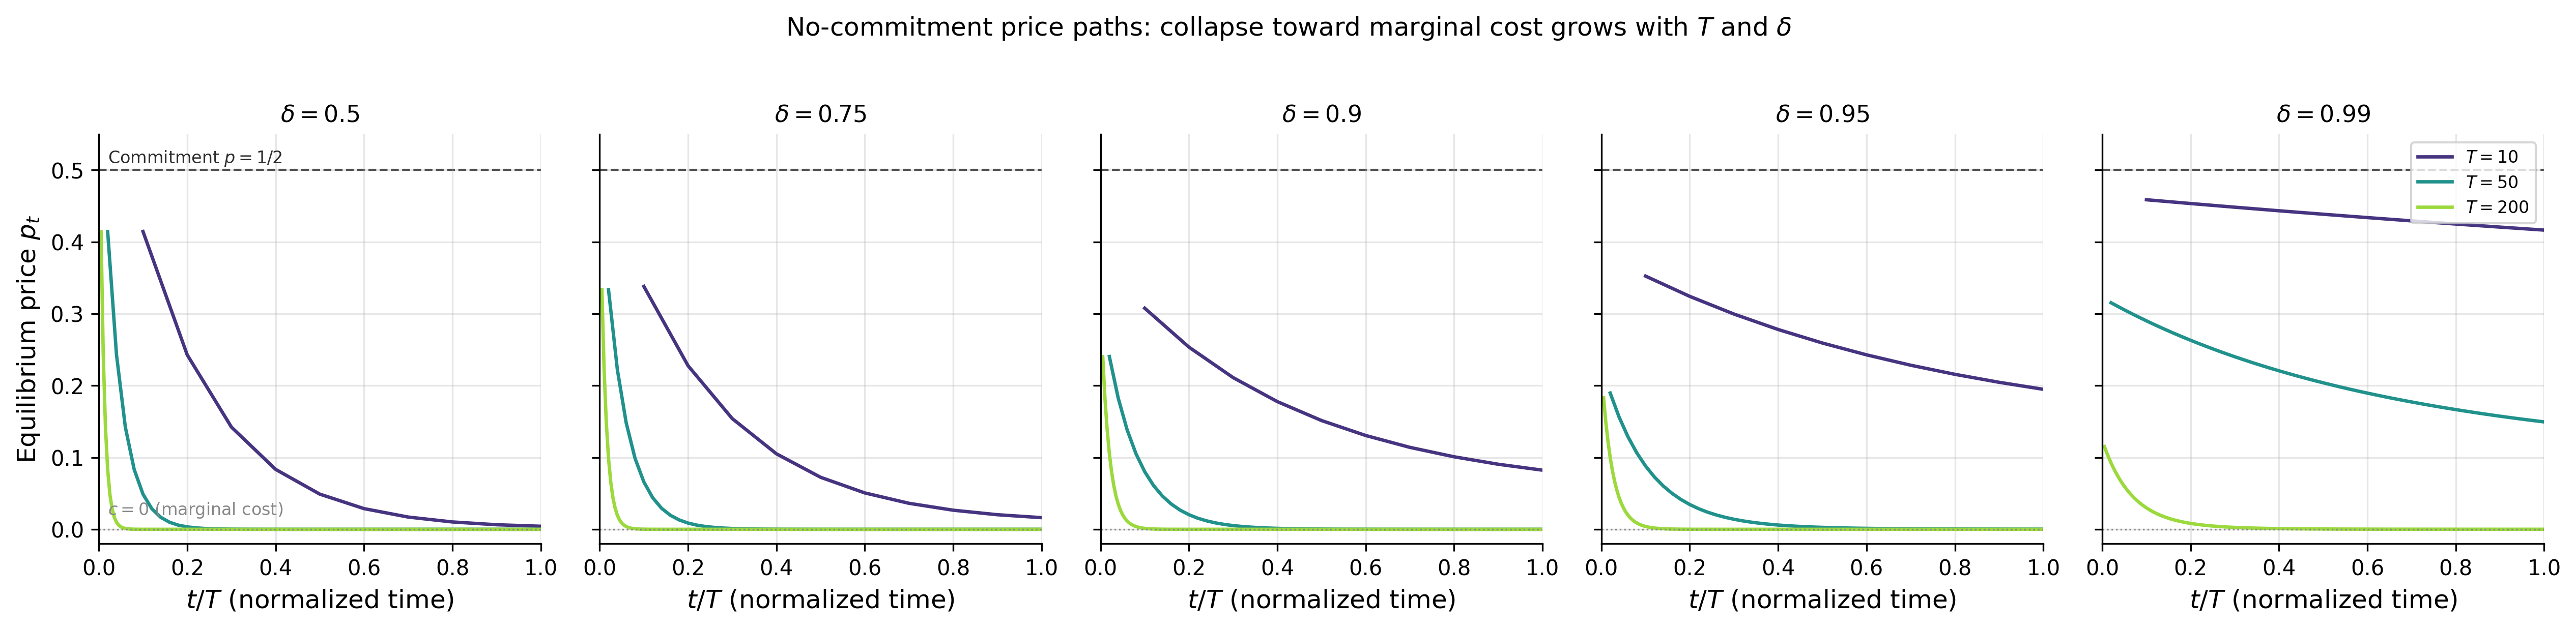
\includegraphics[width=\textwidth]{../ch06_games/sims/durable_goods_coase_price_paths.png}
\caption{No-commitment price paths $p_t$ versus normalized period $t/T$ for representative horizons $T \in \{10, 50, 200\}$ at $\delta \in \{0.5, 0.75, 0.9, 0.95, 0.99\}$. Dashed line: commitment price $p = 1/2$. Dotted line: marginal cost $c = 0$.}
\label{fig:coase_paths}
\end{figure}

\begin{figure}[htbp]
\centering
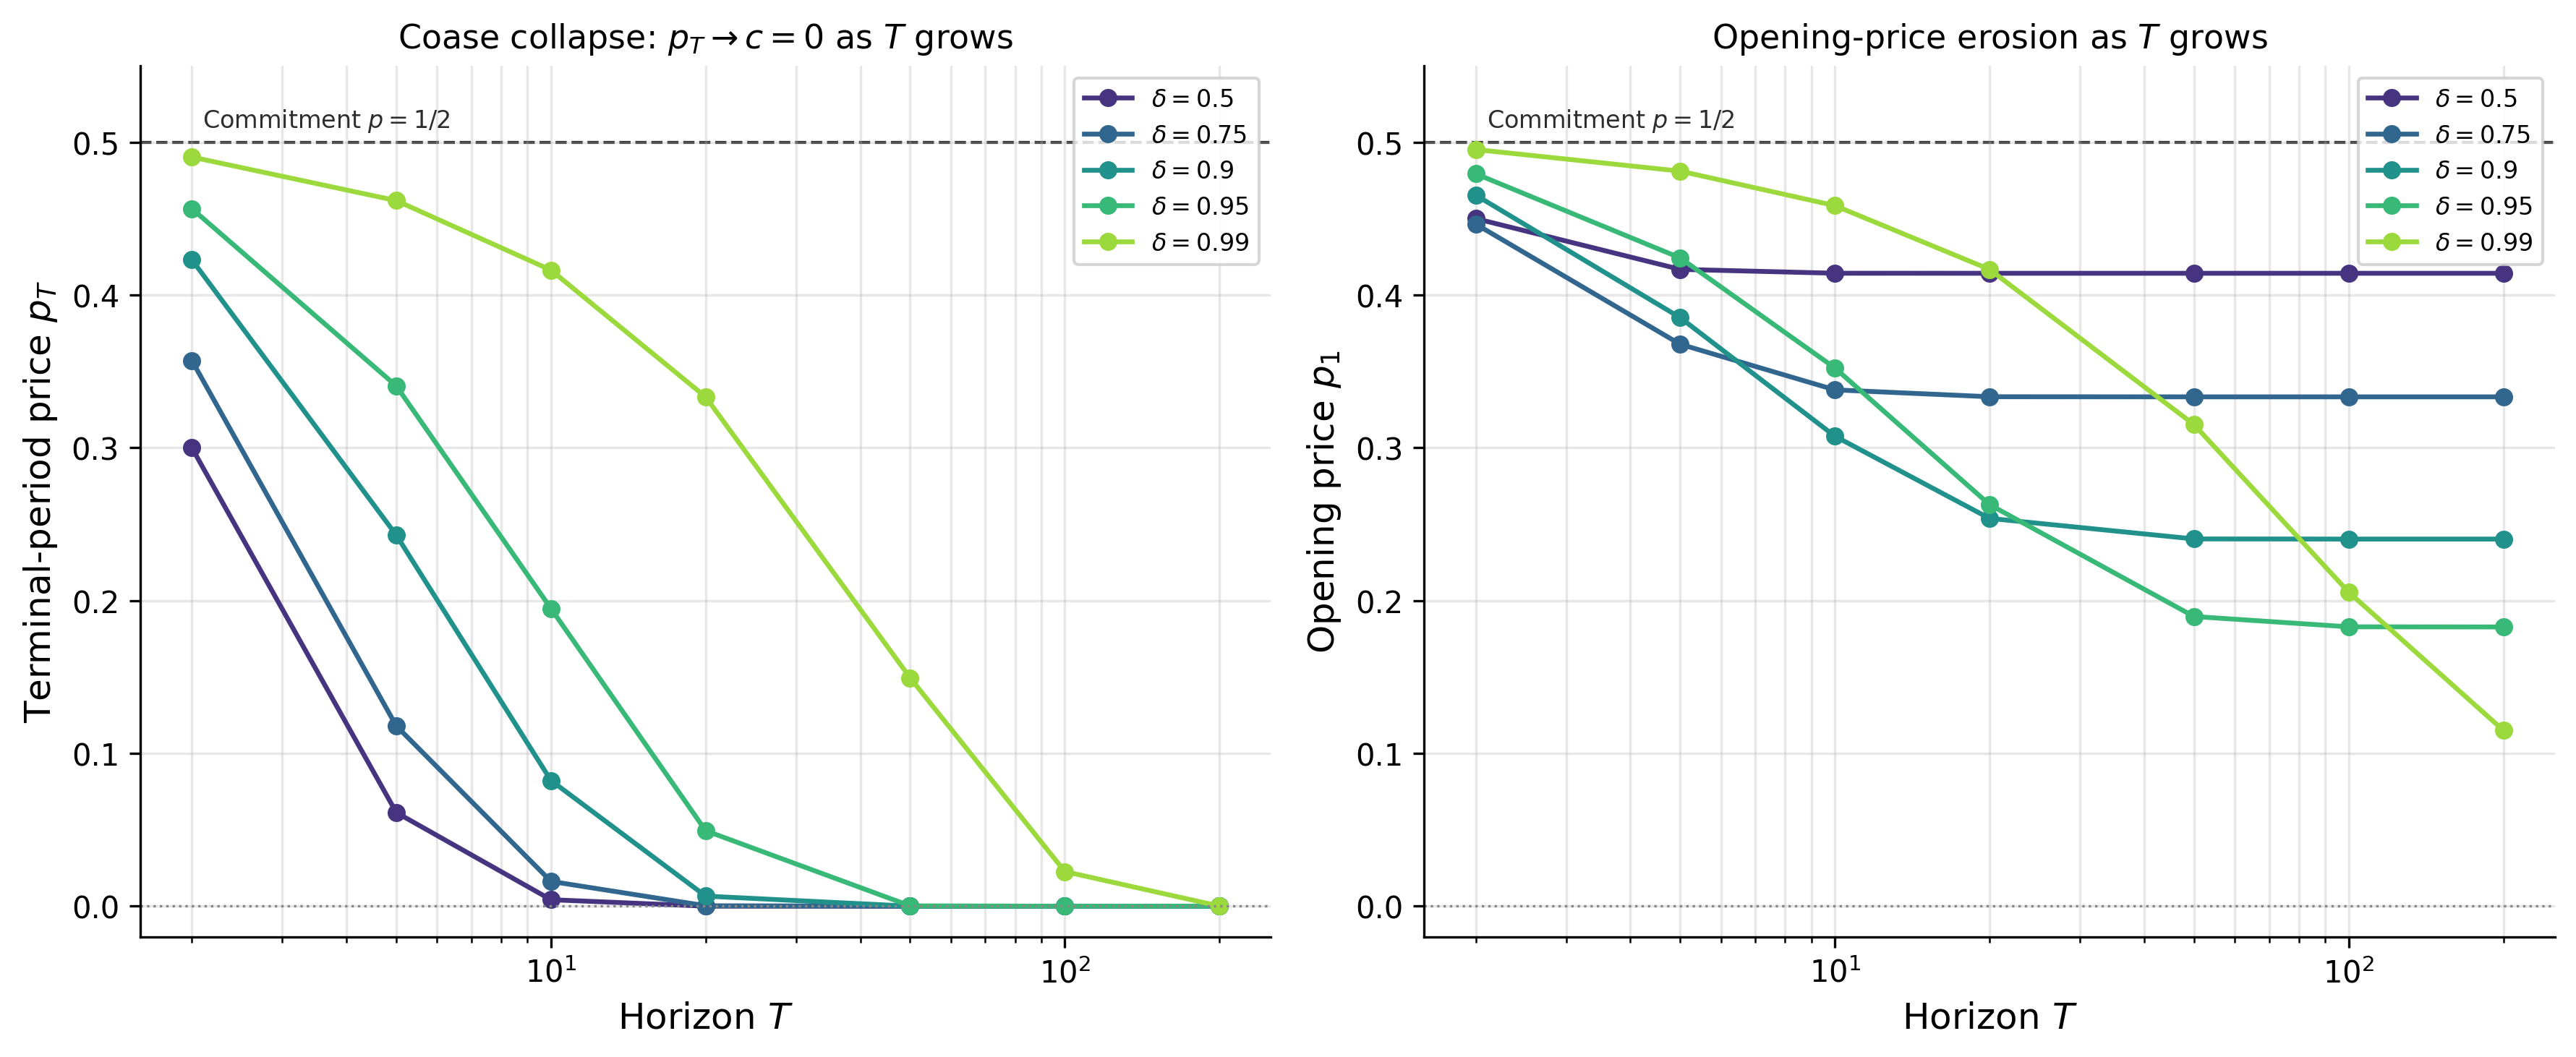
\includegraphics[width=\textwidth]{../ch06_games/sims/durable_goods_coase_collapse.png}
\caption{Coase collapse. Left: terminal-period price $p_T$ versus $T$ on a log-$T$ axis. Right: opening price $p_1$ versus $T$, same axis. Each curve fixes $\delta$.}
\label{fig:coase_collapse}
\end{figure}

\begin{table}[htbp]
\centering
\caption{Commitment value $V^{\mathrm{com}}$, no-commitment Markov-perfect value $V^{\mathrm{nc}}$, ratio $V^{\mathrm{nc}}/V^{\mathrm{com}}$, opening price $p_1$, and terminal price $p_T$ across the $(T, \delta)$ grid. Uniform valuations on $[0, 1]$, $c = 0$.}
\label{tab:coase_dp}
\begin{tabular}{ccccccc}
\toprule
$T$ & $\delta$ & $V^{\mathrm{com}}$ & $V^{\mathrm{nc}}$ & $V^{\mathrm{nc}}/V^{\mathrm{com}}$ & $p_1$ & $p_T$ \\
\midrule
2 & 0.50 & 0.2500 & 0.2250 & 0.900 & 0.4500 & 0.3000 \\
2 & 0.75 & 0.2500 & 0.2232 & 0.893 & 0.4464 & 0.3571 \\
2 & 0.90 & 0.2500 & 0.2327 & 0.931 & 0.4654 & 0.4231 \\
2 & 0.95 & 0.2500 & 0.2397 & 0.959 & 0.4793 & 0.4565 \\
2 & 0.99 & 0.2500 & 0.2476 & 0.990 & 0.4952 & 0.4903 \\
\midrule
5 & 0.50 & 0.2500 & 0.2084 & 0.834 & 0.4168 & 0.0613 \\
5 & 0.75 & 0.2500 & 0.1839 & 0.736 & 0.3678 & 0.1180 \\
5 & 0.90 & 0.2500 & 0.1926 & 0.770 & 0.3852 & 0.2428 \\
5 & 0.95 & 0.2500 & 0.2121 & 0.849 & 0.4243 & 0.3405 \\
5 & 0.99 & 0.2500 & 0.2405 & 0.962 & 0.4811 & 0.4618 \\
\midrule
10 & 0.50 & 0.2500 & 0.2071 & 0.828 & 0.4142 & 0.0042 \\
10 & 0.75 & 0.2500 & 0.1690 & 0.676 & 0.3379 & 0.0162 \\
10 & 0.90 & 0.2500 & 0.1538 & 0.615 & 0.3076 & 0.0823 \\
10 & 0.95 & 0.2500 & 0.1761 & 0.705 & 0.3523 & 0.1948 \\
10 & 0.99 & 0.2500 & 0.2293 & 0.917 & 0.4585 & 0.4163 \\
\midrule
20 & 0.50 & 0.2500 & 0.2071 & 0.828 & 0.4142 & 0.0000 \\
20 & 0.75 & 0.2500 & 0.1667 & 0.667 & 0.3334 & 0.0003 \\
20 & 0.90 & 0.2500 & 0.1269 & 0.508 & 0.2538 & 0.0066 \\
20 & 0.95 & 0.2500 & 0.1314 & 0.526 & 0.2628 & 0.0494 \\
20 & 0.99 & 0.2500 & 0.2084 & 0.834 & 0.4168 & 0.3333 \\
\midrule
50 & 0.50 & 0.2500 & 0.2071 & 0.828 & 0.4142 & 0.0000 \\
50 & 0.75 & 0.2500 & 0.1667 & 0.667 & 0.3333 & 0.0000 \\
50 & 0.90 & 0.2500 & 0.1202 & 0.481 & 0.2404 & 0.0000 \\
50 & 0.95 & 0.2500 & 0.0948 & 0.379 & 0.1896 & 0.0002 \\
50 & 0.99 & 0.2500 & 0.1576 & 0.630 & 0.3152 & 0.1494 \\
\midrule
100 & 0.50 & 0.2500 & 0.2071 & 0.828 & 0.4142 & 0.0000 \\
100 & 0.75 & 0.2500 & 0.1667 & 0.667 & 0.3333 & 0.0000 \\
100 & 0.90 & 0.2500 & 0.1201 & 0.481 & 0.2403 & 0.0000 \\
100 & 0.95 & 0.2500 & 0.0914 & 0.366 & 0.1828 & 0.0000 \\
100 & 0.99 & 0.2500 & 0.1028 & 0.411 & 0.2056 & 0.0227 \\
\midrule
200 & 0.50 & 0.2500 & 0.2071 & 0.828 & 0.4142 & 0.0000 \\
200 & 0.75 & 0.2500 & 0.1667 & 0.667 & 0.3333 & 0.0000 \\
200 & 0.90 & 0.2500 & 0.1201 & 0.481 & 0.2403 & 0.0000 \\
200 & 0.95 & 0.2500 & 0.0914 & 0.365 & 0.1827 & 0.0000 \\
200 & 0.99 & 0.2500 & 0.0576 & 0.230 & 0.1151 & 0.0000 \\
\bottomrule
\end{tabular}
\end{table}

Table~\ref{tab:coase_dp} reports the sweep. At $T = 200$, $\delta = 0.99$ the no-commitment monopolist captures $V^{\mathrm{nc}} = 0.058$ against the commitment benchmark $V^{\mathrm{com}} = 0.25$, a ratio of $0.23$; the terminal price $p_T$ rounds to zero to four decimals, and the opening price $p_1 = 0.115$ is well below the static monopoly price $1/2$. Holding $\delta$ at $0.95$ and varying $T$, the value ratio drops monotonically from $0.96$ at $T = 2$ to $0.37$ at $T = 200$, and $p_T$ from $0.46$ to numerical zero. Holding $T$ at $200$ and varying $\delta$, the ratio drops monotonically from $0.83$ at $\delta = 0.5$ to $0.23$ at $\delta = 0.99$. As a cross-check, the finite-horizon values at $T = 200$ for $\delta \le 0.95$ match the analytical stationary Markov-perfect equilibrium values $\beta^*$ and $\mu^*$ to five decimals.\footnote{The stationary fixed point of the recursion in the footnote above satisfies $\mu = \lambda (1 - \delta) / (1 - \delta \lambda)$, $\beta = \lambda(1-\lambda) A / (1 - \delta \lambda^2)$, and $\lambda = A / (2 (A - \delta \beta))$. At $\delta = 0.9$ this gives $\lambda \approx 0.760$, $\mu \approx 0.240$, $\beta \approx 0.120$, matching the table's $T = 200$ entries. At $\delta = 0.99$ the stationary $\mu \approx 0.091$, $\beta \approx 0.045$, so $T = 200$ is still slightly above the asymptotic limit; the residual gap closes as $T$ grows further.}

Figure~\ref{fig:coase_paths} traces the equilibrium price path: long horizons and patient buyers force the seller to start lower and end near marginal cost. Figure~\ref{fig:coase_collapse} summarizes the collapse rate: $p_T \to 0$ at all $\delta < 1$ once $T$ is large enough, and $p_1$ falls toward the stationary level $\mu^*(\delta)$ that itself tends to zero as $\delta \to 1$.

The Coase conjecture is delivered numerically: in the absence of commitment power, the durable-goods monopolist captures only a fraction of the commitment surplus, and that fraction shrinks toward zero as $T$ and $\delta$ jointly grow. Section~\ref{subsec:durable_goods_screening} below presents a two-period precursor that focuses on the screening-versus-pooling equilibrium structure.

\subsection{Screening versus Pooling in the Durable Goods Monopoly}
\label{subsec:durable_goods_screening}

The two-period analogue of the model in Section~\ref{subsec:coase} reduces to an extensive-form game with a discrete buyer type and a discrete seller action set; it is small enough to admit equilibrium computation via counterfactual regret minimization (CFR) and serves as a methodological precursor to the dynamic programming sweep above. Replacing the continuum of valuations with a two-point distribution $v \in \{v_L, v_H\}$ and restricting the seller to two prices $\{v_L, P^*(\delta)\}$ recovers the screening-versus-pooling threshold $\pi^* = 1/2$ in closed form; CFR finds this threshold without being told the analytical solution.

\subsubsection{Model}

A seller with zero cost faces a buyer with private valuation $v \in \{v_L, v_H\}$, where $\Pr(v = v_H) = \pi$. In each period $t = 1, 2, \ldots$, the seller posts price $p_t$; the buyer accepts or rejects. Upon acceptance at $t$, the seller receives $\delta^{t-1} p_t$ and the buyer receives $\delta^{t-1}(v - p_t)$, where $\delta \in (0,1)$ is the common discount factor. The game ends upon acceptance or after $T$ periods. Parameters: $v_L = 100$, $v_H = 200$, $T = 2$ periods.

\subsubsection{Equilibrium Analysis}

The screening price $P^*(\delta)$ makes the high-type buyer indifferent between accepting now and waiting.
\begin{equation}
v_H - P^* = \delta(v_H - v_L) \implies P^*(\delta) = v_H - \delta(v_H - v_L).
\end{equation}
The seller's optimal strategy depends on $\pi$. Let $\Pi_{\text{screen}} = \pi P^* + (1-\pi)\delta v_L$ and $\Pi_{\text{pool}} = v_L$. The seller screens if $\Pi_{\text{screen}} > \Pi_{\text{pool}}$, yielding threshold
\begin{equation}
\pi^* = \frac{v_L(1-\delta)}{P^* - \delta v_L} = \frac{1}{2} \quad \text{when } v_H = 2v_L.
\end{equation}
For $\pi < \pi^*$, the seller pools (offers $v_L$ immediately). For $\pi > \pi^*$, the seller screens (offers $P^*$, then $v_L$ if rejected).\footnote{In a screening equilibrium, the seller uses price to separate buyer types: high-value buyers accept immediately at a high price, while low-value buyers reject and receive a lower offer. In a pooling equilibrium, the seller offers a single price that all types accept. The gap case ($0 = c < v_L$) guarantees trade in equilibrium.} As $\delta \to 1$, the screening price $P^*(\delta) \to v_L$ and the seller cannot extract a screening premium from high types, but in a two-period game with action set $\{v_L, P^*(\delta)\}$ the asymptotic price-collapse mechanism of the Coase conjecture does not operate.

\subsubsection{Computational Results}

I model the bargaining game as an extensive-form game and apply CFR.\footnote{The game tree has two information sets for the seller (indexed by rejection history) and two for the buyer (indexed by private type). CFR runs for 5,000 iterations per parameter configuration. Vanilla CFR is deterministic given zero initial regrets, so seed-level variability is obtained by perturbing the initial regret table with small Gaussian noise (standard deviation $0.05$); ten seeds are run per $(\pi, \delta)$ cell. The reported P(Screen) and NashConv are means across seeds; SE columns report the standard error of the mean. NashConv is the sum of both players' exploitabilities, reported on the utility scale where the maximum single-player payoff is $v_H = 200$.}

\begin{table}[htbp]
\centering
\caption{CFR strategy versus analytical equilibrium: $\pi$-sweep at $\delta = 0.5$, $n = 10$ seeds per cell.}
\label{tab:coase}
\begin{tabular}{lcccccccc}
\toprule
$\pi$ & $P^*$ & P(Screen) & SE & Theory & $|\Delta|$ & NashConv & SE & Eq.\ Type \\
\midrule
0.10 & 150 & 0.000 & 0.000 & 0.0 & 0.000 & 4.04 & 0.59 & Pooling \\
0.15 & 150 & 0.000 & 0.000 & 0.0 & 0.000 & 6.04 & 0.88 & Pooling \\
0.20 & 150 & 0.000 & 0.000 & 0.0 & 0.000 & 8.04 & 1.17 & Pooling \\
0.25 & 150 & 0.000 & 0.000 & 0.0 & 0.000 & 10.05 & 1.46 & Pooling \\
0.30 & 150 & 0.001 & 0.000 & 0.0 & 0.001 & 12.05 & 1.75 & Pooling \\
0.35 & 150 & 0.001 & 0.000 & 0.0 & 0.001 & 14.06 & 2.04 & Pooling \\
0.40 & 150 & 0.001 & 0.001 & 0.0 & 0.001 & 16.58 & 2.37 & Pooling \\
0.45 & 150 & 0.202 & 0.133 & 0.0 & 0.202 & 23.36 & 4.80 & Pooling \\
0.50 & 150 & 0.351 & 0.150 & 0.5 & 0.149 & 23.85 & 4.32 & Indifferent \\
0.55 & 150 & 0.401 & 0.163 & 1.0 & 0.599 & 23.59 & 3.97 & Screening \\
0.60 & 150 & 0.598 & 0.144 & 1.0 & 0.402 & 23.20 & 3.78 & Screening \\
0.65 & 150 & 0.801 & 0.132 & 1.0 & 0.199 & 22.41 & 3.11 & Screening \\
0.70 & 150 & 0.900 & 0.100 & 1.0 & 0.100 & 19.41 & 2.75 & Screening \\
0.75 & 150 & 0.900 & 0.100 & 1.0 & 0.100 & 16.16 & 2.29 & Screening \\
0.80 & 150 & 1.000 & 0.000 & 1.0 & 0.000 & 14.92 & 1.27 & Screening \\
0.85 & 150 & 1.000 & 0.000 & 1.0 & 0.000 & 11.17 & 0.96 & Screening \\
0.90 & 150 & 1.000 & 0.000 & 1.0 & 0.000 & 7.42 & 0.65 & Screening \\
\bottomrule
\end{tabular}
\begin{minipage}{0.9\textwidth}
\footnotesize
Notes: P(Screen) is the probability the seller offers $P^* = 150$ in period 1, averaged across seeds. SE columns report the across-seed standard error. Theory gives the analytical pure-strategy prediction (0 for pooling, 1 for screening, 0.5 at the indifference point $\pi^* = 1/2$). $|\Delta| = |\text{P(Screen)} - \text{Theory}|$. NashConv is the sum of both players' exploitabilities at iteration 5000, on the same utility scale as the payoffs.
\end{minipage}
\end{table}

Table~\ref{tab:coase} reports results from varying $\pi$ at fixed $\delta = 0.5$. Away from the indifference threshold ($\pi \le 0.40$ and $\pi \ge 0.80$), CFR's average strategy matches the analytical step function: $|\Delta| \le 0.001$ in the pooling region and $|\Delta| = 0.000$ in the deep screening region. In the transition window $\pi \in [0.45, 0.65]$, CFR returns mixed strategies with across-seed standard errors of $0.13$--$0.16$, reflecting the seller's economic indifference where both pooling and screening yield identical expected profit. The empirical transition CFR finds is slightly delayed relative to the analytical $\pi^* = 1/2$: $\text{P(Screen)} \approx 0.60$ at $\pi = 0.60$ and reaches $0.90$ only at $\pi = 0.70$. Residual NashConv after 5{,}000 iterations is in the range $4$--$24$ across $\pi$, equivalent to up to $12\%$ of the maximum single-player payoff; CFR is not at $\varepsilon$-Nash for small $\varepsilon$ here, and reporting NashConv on a linear utility scale rather than a log scale makes this gap visible.

A $\delta$-sweep at $\pi = 0.7$ verifies the screening price formula $P^*(\delta) = 200 - 100\delta$ with zero error across $\delta \in [0.1, 0.9]$. The CFR average P(Screen) drops from $1.0$ at $\delta = 0.1$ to $0.50 \pm 0.17$ at $\delta \ge 0.75$. The analytical column predicts pure screening (P(Screen) $= 1$) throughout this range because $\pi = 0.7 > \pi^* = 1/2$, so this drift is not a Coase regime switch. Instead, as $\delta$ grows, the screening price $P^*(\delta)$ shrinks toward $v_L$ and the seller's screening profit approaches the pooling profit; the seller becomes near-indifferent and CFR's average strategy spreads across the two corners under seed-perturbed initial regrets.\footnote{Four stress tests were conducted: (1) awkward primes $(v_L, v_H) = (37, 83)$, converging to $P^* = 55$ (theory: 55.4); (2) information leak with a single seller information set at the root; (3) grid shift with 150 removed, recovering 145 (99.4\%); (4) 3-period game, finding $P_1 = 120$ versus theoretical 136. The 3-period result reflects a tie-breaking equilibrium: at $P_1 = 136$ the high buyer is exactly indifferent, so the seller prefers $P_1 = 120$ (revenue 108 versus 86.4 if rejected).}

\subsection{Discussion}

Stochastic-game Q-learning and CFR target complementary game classes: simultaneous-move games with observable payoffs and extensive-form games with private information, respectively. The simulations confirm convergence to known equilibria in both settings without encoding domain structure into the algorithms.
